\documentclass[sectionformat=aufgabe]{gadsescript}

\setsemester{Summer Semester 2024}%
\setuniversity{University of Konstanz}%
\settitlelh{\today\\\semester\\Gruppe 3, Jonathan Weihing}
\setfaculty{Faculty of Science\\(Mathematics and Statistics)}%
\settitle{Übungsblatt 6}
\setsubtitle{Elias Gestrich}
\usepackage{subfig}

\begin{document}
\maketitle
Schreibweise: bei
\[
	\lim_{h \to 0} 
\]
ist immer
\[
	\lim_{\overset{h\to 0}{h\neq 0}} 
\]
gemeint

\section{Differenzierbarkeit von Normen}
Es sei $ \left\| \cdot  \right\|  $ eine (beliebige) Norm auf $ \R ^n $. Zeigen Sie, dass
\begin{enumerate}[label=(\alph*)]
	\item $ \left\| \cdot  \right\|  $ nicht differenzierbar in $ 0 \coloneqq \left( 0, \dotsc, 0 \right) ^T $ ist.
	\item für jedes $ \varepsilon > 0 $ die Funktionen $ x \mapsto \left\| x \right\| ^{1 + \varepsilon }  $ differenzierbar in $ 0 $ ist.
\end{enumerate}

\textbf{Bew.:}\\
\begin{enumerate}[label=(\alph*)]
	\item Betrachte
		\[
			\lim_{\underset{h < 0}{h \nearrow 0}} \frac{ \left\| h \right\| - \left\| 0 \right\| }{ h } = \frac{\left| h \right| }{ h } \left\| 1 \right\| = - \left\| 1 \right\| < 0
		\]
		und
		\[
			\lim_{\underset{h > 0}{h \searrow 0}} \frac{ \left\| h \right\| - \left\| 0 \right\| }{ h } = \frac{\left| h \right| }{ h } \left\| 1 \right\| = \left\| 1 \right\| > 0
		\]
		Somit existiert kein allgemeiner Grenzwert und $ \left\| \cdot  \right\|  $ ist nicht am Punkt $ 0 $ differenzierbar
	\item Nach Definition 4.1 ist $ \left\| \cdot  \right\| ^{1 + \varepsilon }  $ genau dann differenzierbar, wenn
		\[
			\lim_{\underset{h \neq 0}{h \to 0}} \frac{ \left\| h \right\| ^{1 + \varepsilon } - \left\| 0 \right\| ^{1 + \varepsilon }  - L(h) }{ \left| h \right|  } = 0.
		\]
		Setze $ L \coloneqq 0 $ und betrachte den Limes:
		\begin{align*}
			\lim_{\underset{h \neq 0}{h \to 0}} \frac{ \left| \left\| h \right\| ^{1 + \varepsilon } - \left\| 0 \right\| ^{1 + \varepsilon } \right| }{ \left\| h \right\|  } &= \lim_{\underset{h \neq 0}{h \to 0}} \frac{ \left| \left| h \right| ^{1 + \varepsilon } \left\| 1 \right\| ^{1 + \varepsilon } \right| }{ \left| h \right|  }  \\
			~ &= \left\| 1 \right\|  \lim_{\underset{h \neq 0}{h \to 0}} \left\| h \right\| ^{\varepsilon } \\
			~ &= 0 \left\| 1 \right\| \\
			~ &= 0
		\end{align*}
\end{enumerate}

\section{Nicht stetige partielle Ableitungen}
Betrachten Sie die Funktion $ f : \R ^2 \to \R  $ definiert durch
\[
	f(x, y) \coloneqq \begin{cases}
		(x^2 + y^2) \sin \left( \frac{ 1 }{ x^2 + y^2 }  \right) , &(x, y) \neq (0, 0),\\
		0, &\text{sonst.} 
	\end{cases}
\]
Zeigen Sie: $ f $ ist differenzierbar, die partiellen Ableitungen von $ f $ sind aber nicht stetig.

Differenzierbar:\\
Sei $ g : \R ^2 \to \R , g(x, y) \to x^2 + y^2 $.
Beh.: $ g $ differenzierbar.
Setze dafür $ L_g(h_x, h_y) \coloneqq 2xh_x + 2yh_y $ so, dass
\begin{align*}
	~&\lim_{(h_x, h_y) \to (0, 0)} \frac{ \left| g(x + h_x, y + h_y) - g(x, y) - L_g(h_x, h_y) \right| }{ \left\| h \right\|_2  } \\
	=& \lim_{(h_x, h_y) \to (0, 0)} \frac{ \left| (x + h_x)^2 + (y + h_y)^2 - x^2 - y^2 - 2xh_x - 2yh_y \right| }{ \left\| h \right\|_2  }  \\
	=& \lim_{(h_x, h_y) \to (0, 0)} \frac{ \left| x^2 + 2xh_x + h_x^2 + y^2 + 2yh_y + h_y^2 - x^2 - y^2 - 2xh_x - 2yh_y \right| }{ \left\| h \right\|_2  }  \\
	=& \lim_{(h_x, h_y) \to (0, 0)} \frac{ \left| h_x^2 + h_y^2 \right| }{ \left\| h \right\|_2  }  \\
	=& \lim_{(h_x, h_y) \to (0, 0)} \frac{ \left\| (h_x, h_y) \right\| _2^2 }{ \left\| h \right\|_2  }  \\
	=& \lim_{(h_x, h_y) \to (0, 0)} \left\| (h_x, h_y) \right\| _2 \\
	=& \lim_{(h_x, h_y) \to (0, 0)} 0
\end{align*}

Daraus folgt nach Ana I, dass $ \frac{ 1 }{ g(x, y) }  $ differenzierbar, für $ g(x, y) \neq 0 $, also $ (x, y) \neq (0, 0) $.
Also auch $ \sin \left( \frac{ 1 }{ g(x, y) }  \right)  $ differenzierbar, für $ (x, y) \neq (0, 0) $.
Und $ g(x, y) \cdot \sin \left( \frac{ 1 }{ g(x, y) }  \right)  $ differenzierbar für $ (x, y) \neq (0, 0) $.
Noch zu zeigen $ f(x, y) $ differenzierbar an der Stelle $ (0, 0) $:
Setze $ L(h) \coloneqq 0 $:
\begin{align*}
	\lim_{(h_x, h_y) \to (0, 0)} \frac{ \left| f(0 + h_x, 0 + h_y) - f(0, 0) - 0 \right| }{ \left\| (h_x, h_y) \right\|_2  } &= \lim_{(h_x, h_y) \to (0, 0)} \frac{ \left| (h_x^2 + h_y)^2 \sin \left( \frac{ 1 }{ (h_x^2 + h_y^2) }  \right) \right| }{ \left\| (h_x, h_y) \right\|_2  }  \\
	&= \lim_{(h_x, h_y) \to (0, 0)} \frac{ \left\| (h_x, h_y) \right\|_2^2 \left| \sin \left( \frac{ 1 }{ (h_x^2 + h_y^2) }  \right) \right| }{ \left\| (h_x, h_y) \right\|_2  }  \\
	&\leq  \lim_{(h_x, h_y) \to (0, 0)} \left\| (h_x, h_y) \right\|_2 \\
	&= 0
\end{align*}

Nach Ana I sind die partiellen Ableitungen wie folgt:
\begin{align*}
	\frac{ \partial }{ \partial x } f(x, y) &= 2x \sin \left( \frac{ 1 }{ x^2 + y^2 }  \right) - \frac{ 2x }{ x^2 + y^2 } \cos \left( \frac{ 1 }{ x^2 + y^2 }  \right) \\
						&= 2x \left( \sin \left( \frac{ 1 }{ x^2 + y^2 } \right) - \frac{ \cos \left( \frac{ 1 }{ x^2 + y^2 }  \right) }{ x^2 + y^2 } \right)
\end{align*}
\begin{align*}
	\frac{ \partial }{ \partial y } f(x, y) &= 2y \sin \left( \frac{ 1 }{ x^2 + y^2 }  \right) - \frac{ 2y }{ x^2 + y^2 } \cos \left( \frac{ 1 }{ x^2 + y^2 }  \right) \\
						&= 2y \left( \sin \left( \frac{ 1 }{ x^2 + y^2 } \right) - \frac{ \cos \left( \frac{ 1 }{ x^2 + y^2 }  \right) }{ x^2 + y^2 } \right)
\end{align*}
Dann für $ y = 0 $ und $ x_j \coloneqq \sqrt{ \frac{ 1 }{ j_2 \pi  } }  $:
\begin{align*}
	~ & 2x_j \sin \left( \frac{ 1 }{ x_j^2 }  \right) - \frac{ 2x_j }{ x_j^2 } \cos \left( \frac{ 1 }{ x_j^2 }  \right) \\
	=& 2 \sqrt{ \frac{ 1 }{ j 2\pi } } \sin ( j 2\pi ) - 2 \sqrt{ j 2 \pi } \cos ( j 2\pi ) \\
	=& -2 \sqrt{j 2\pi } \\
	=& -\infty
\end{align*}
Aber für $ y = 0 $ und $ x_j \coloneqq \sqrt{ \frac{ 1 }{ \frac{ \pi }{ 2 } + j 2\pi  } } $:
\begin{align*}
	&\lim_{j \to \infty} 2x_j \sin \left( \frac{ 1 }{ x_j^2 }  \right) - \frac{ 2x_j }{ x_j^2 } \cos \left( \frac{ 1 }{ x_j^2 }  \right)\\
	=& \lim_{j \to \infty} 2 \sqrt{ \frac{ 1 }{ \frac{ \pi }{ 2 } + j 2\pi } } \sin ( \frac{ \pi }{ 2 } + j 2\pi ) - 2 \sqrt{ \frac{ \pi }{ 2 } + j 2\pi } \cos ( \frac{ \pi }{ 2 } + j 2\pi ) \\
	= & \lim_{j \to \infty} 2 \sqrt{ \frac{ 1 }{ \frac{ \pi }{ 2 } + j 2\pi  }  } \\
	= & 0
\end{align*}
Wenn es stetig wäre, müsste das selbe rauskommen (Folgenstetig)

Für $ \frac{ \partial }{ \partial y } f(x, y) $ analog


\section{Richtungsableitugnen und Differenzierbarkeit}
Betrachten Sie die Funktion
\[
	f: \R ^2 \to \R , (x, y) \mapsto \begin{cases}
		\frac{ 2 x^2 y }{ x^2 + y^2 } , & (x, y) \neq (0, 0),\\
		0, & (x, y) = (0, 0)
	\end{cases}
\]
Zeigen Sie: $ f $ ist stetig und für $ f $ existieren alle Richtungsableitungen an der Stelle $ (0, 0) $, aber $ f $ ist nicht differenzierbar in $ (0, 0) $.

Zu zeigen für $ (x_j, y_j) \to (x_0, y_0) $ konvergiert $ f(x_j, y_j)  $ gegen $ f(x_0, y_0) $.
Für $ (x_0, y_0) = (0, 0) $ und $ x_j \neq 0 $
\begin{align*}
	\lim_{j \to \infty} \left| \frac{ 2 x_j^2 y_j }{ x_j^2 + y_j^2 }  \right|
	&\leq \lim_{j \to \infty} \left| \frac{ 2 x_j^2 y_j }{ x_j^2 }  \right|  \\
	&\leq \lim_{j \to \infty} \left| 2 y_j \right| \\
	&= 0
\end{align*}
Für $ x_j = 0 $, dann ist bereits $ f(x_j, y_j) = 0 = f(x_0, y_0) $.

Für $ (x_0, y_0) \neq (0, 0) $ 
\[
	\lim_{j \to \infty} f(x_j, y_j) = \lim_{j \to \infty} \frac{ 2 x_j^2 y_j }{ x_j^2 + y_j^2 } \overset{\text{Ana I} }{=} \frac{2 x^2 y^2 }{ x_0^2 + y_0^2 } = f(x_0, y_0)
\]
Was zu zeigen war.

Richtungsableitung:
Sei $ \nu \in \R ^2 $, sodass $ \nu = (\nu_x, \nu_y) \neq (0, 0) $. Zu zeigen
\[
	\lim_{h \to 0} \frac{ f(h\nu_x, h\nu_y) - f(0, 0) }{ h } 
\]
konvergiert.

\begin{align*}
	\lim_{h \to 0}  \frac{f(h\nu_x, h\nu_y) - 0 }{ h } &= \frac{2(h\nu_x)^2 h\nu_y}{ h ((h \nu_x)^2 + (h \nu_y)^2 } \\
	&= \frac{2h^3\nu_x^2\nu_y}{ h^3(\nu_x^2 + \nu_y^2 }  \\
	&= \frac{2\nu_x^2\nu_y}{ \nu_x^2 + \nu_y^2 }  \\
\end{align*}
Insbesondere für $ \nu = (1, 0) $ oder $ \nu = (0, 1) $ ist die Richtungsableitung $ 0 $.

Nicht differenzierbar an $ (0, 0) $: Nach Definition 4.1
$ L(h) = \nabla f(x, y) \cdot h = 0 $.
Also reicht zu zeigen
\[
	\lim_{h \to 0} \frac{ \left| f(h, h) - f(0, 0) - 0 \right|}{ \left| (h, h) \right|  } \neq 0
\]
\begin{align*}
	\lim_{(h, h) \to (0, 0)} \frac{ \left| f(h, h) - f(0, 0) - 0 \right|}{ \left\| (h, h) \right\|_2  } &= \lim_{(h, h) \to (0, 0)} \frac{\left| f(h, h) \right| }{ \left\| h, h \right\|_2  }  \\
	&= \lim_{h \to 0}  \left| \frac{ 2h^2h }{ (h^2 + h^2)\sqrt{h^2 + h^2}  } \right| \\
	&= \lim_{h \to 0} \left| \frac{ 2h^3 }{ 2h^3\sqrt{2}  } \right| \\
	&= \lim_{h \to 0} \left| \frac{ 2 }{ 2\sqrt{2}  } \right| \\
	&= \lim_{h \to 0} \frac{ \sqrt{2}  }{ 2 } \\
	&= \frac{ \sqrt{2}  }{ 2 } \\
	&> 0
\end{align*}

%\[
%	\frac{ \partial }{ \partial x } f(x, y) = \frac{ ( 4 x y ) (x^2 + y^2) - (2x^2 y ) ( 2x) }{ (x^2 + y^2)^2 } = \frac{ 4 x y^3 }{ (x^2 + y^2)^2 } 
%\]
%\[
%	\frac{ \partial }{ \partial y } f(x, y) = \frac{ ( 2 x^2 ) (x^2 + y^2) - (2x^2 y ) ( 2y) }{ (x^2 + y^2)^2 } = \frac{ 2 x^4 - 2 x^2 y^2 }{ (x^2 + y^2)^2 } 
%\]



\section{Vertauschen von partiellen Ableitungen}
Sei die Funktion $ f : \R ^2 \to \R  $ definiert durch
\[
	f(x) \coloneqq 
	\begin{cases}
		x_1x_2 \frac{x_1^2 - x_2^2}{ \left| x \right| ^2 } , & x \neq 0,\\
		0, & x = 0
	\end{cases}
\]
für $ x = (x_1, x_2)^T \in \R ^2 $. Zeigen Sie, dass alle partiellen Ableitungen bis zum Grad 2 existieren.
Zeigen Sie außerdem, dass $ \partial_1 \partial_1 f(0) \neq \partial_2 \partial_1 f(0) $.
Steht dies im Widerspruch zum Satz von Schwarz?

für $ x \neq 0 $, wende Ableitungsregeln aus Ana I an:
\begin{align*}
	\partial_1 f(x) &= \frac{ ( 3x_1^2 x_2 - x_2^3 ) \left| x \right| ^2 - x_1x_2(x_1^2 - x_2^2) * 2x_1 }{ \left| x \right| ^4 } \\
	~&= \frac{ ( 3x_1^2 x_2 - x_2^3 ) (x_1^2 + x_2^2) - 2(x_1^4x_2 - x_1^2x_2^3) }{ \left| x \right| ^4 } \\
	~&= \frac{ ( 3x_1^4 x_2 - x_1^2x_2^3 + 3x_1^2x_2^3 - y_2^5 ) - 2x_1^4x_2 + 2x_1^2x_2^3 }{ \left| x \right| ^4 } \\
	~&= \frac{ (  x_1^4 x_2 + 4x_1^2x_2^3 - x_2^5 ) }{ \left| x \right| ^4 } \\
	~&= x_2 \frac{ (  x_1^4 + 4x_1^2x_2^2 - x_2^4 ) }{ \left| x \right| ^4 } \\
\end{align*}
\begin{align*}
	\partial_2 f(x) &= \frac{ ( x_1^3 - 3x_1x_2^2 ) \left| x \right| ^2 - x_1x_2(x_1^2 - x_2^2) * 2x_2 }{ \left| x \right| ^4 } \\
	~&= \frac{ ( x_1^3 - 3x_1x_2^2 ) (x_1^2 + x_2^2) - 2(x_1^3x_2^2 - x_1x_2^4) }{ \left| x \right| ^4 } \\
	~&= \frac{ ( x_1^5 - 3x_1^3x_2^2 + x_1^3x_2^2 - 3x_1x_2^4 ) - 2x_1^3x_2^2 + 2x_1x_2^4 }{ \left| x \right| ^4 } \\
	~&= \frac{ ( x_1^5 - 4x_1^3x_2^2 - x_1x_2^4 ) }{ \left| x \right| ^4 } \\
	~&= x_1 \frac{ (  x_1^4 - 4x_1^2x_2^2 - x_2^4 ) }{ \left| x \right| ^4 } \\
\end{align*}
Trivialerweise ist $ \partial_i $ nach $ x_j $ differenzierbar, wende hierfür Ableitungsregeln an.

für $ x = 0 $, sei $ f_1: \R \to \R, x \mapsto  f(x, 0) $ und $ f_2: \R \to \R , x \mapsto f(0, x) $
\begin{align*}
	\lim_{h \to 0} \frac{ f_1(h) - f_1(0) }{ h } &= h \cdot 0 \cdot \frac{h^2 - 0^2}{ h^3 } = 0
\end{align*}
\begin{align*}
	\lim_{h \to 0} \frac{ f_2(h) - f_2(0) }{ h } &= 0 \cdot h \cdot \frac{0^2 - h^2}{ h^3 } = 0
\end{align*}
Also $ \partial_1 f(0) = 0 = \partial_2 f(0) $.
\begin{align*}
	\partial_1 \partial_1 f(0) &= \lim_{h \to 0} \frac{ \partial_1 f(h, 0) - \partial_1 f(0, 0) }{ h } \\
	~ &= \lim_{h \to 0} \frac{ 0 \frac{ h^4 +4h^2 \cdot 0^2 - 0^4 }{ h^4 } - 0 }{ h }\\
	~ &= 0
\end{align*}
\begin{align*}
	\partial_2 \partial_1 f(0) &= \lim_{h \to 0} \frac{ \partial_1 f(0, h) - \partial_1 f(0, 0) }{ h } \\
	~ &= \lim_{h \to 0} \frac{ h \frac{ 0^4 +40^2 \cdot h^2 - h^4 }{ h^4 } - 0 }{ h }\\
	~ &= \lim_{h \to 0} \frac{ h \cdot (-1) }{ h } \\
	~ &= -1
\end{align*}
\begin{align*}
	\partial_1 \partial_2 f(0) &= \lim_{h \to 0} \frac{ \partial_2 f(h, 0) - \partial_2 f(0, 0) }{ h } \\
	~ &= \lim_{h \to 0} \frac{ h \frac{ h^4 +4h^2 \cdot 0^2 - 0^4 }{ h^4 } - 0 }{ h }\\
	~ &= \lim_{h \to 0} \frac{ h }{ h } \\
	~ &= 1
\end{align*}
\begin{align*}
	\partial_2 \partial_2 f(0) &= \lim_{h \to 0} \frac{ \partial_2 f(0, h) - \partial_2 f(0, 0) }{ h } \\
	~ &= \lim_{h \to 0} \frac{ 0 \frac{ 0^4 +40^2 \cdot h^2 - h^4 }{ h^4 } - 0 }{ h }\\
	~ &= 0
\end{align*}

Daraus folgt, dass $ \partial_1\partial_2 f(0) = 1 \neq -1 = \partial_2\partial_1 f(0) $.
Dies steht nicht im Widerspruch zu dem Satz von Schwarz, da hierfür die zweiten partiellen differentiale stetig sein müssen.
Dies ist wahrscheinlich nicht der Fall (sonst würde ja der Satz von Schwarz greifen)

Weil mir langweilig ist:
\begin{figure}[h]
	\subfloat[Aufgabe 2]{
	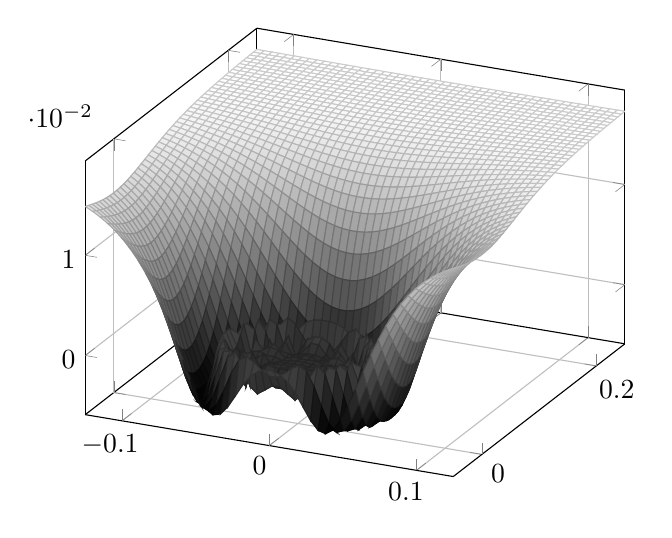
\begin{tikzpicture}
		\begin{axis}[
			domain    = -0.125:0.125,
			samples    = 50,
			y domain  = -0.05:0.25,
			samples y  = 50,
			colormap/blackwhite,
			grid,
			%rotate around x = 30,
			]
			\addplot3[surf] { (x^2 + y^2 ) * sin( 1/(x^2 + y^2) ) };
		\end{axis}
	\end{tikzpicture}
	}
	\subfloat[Aufgabe 3]{
	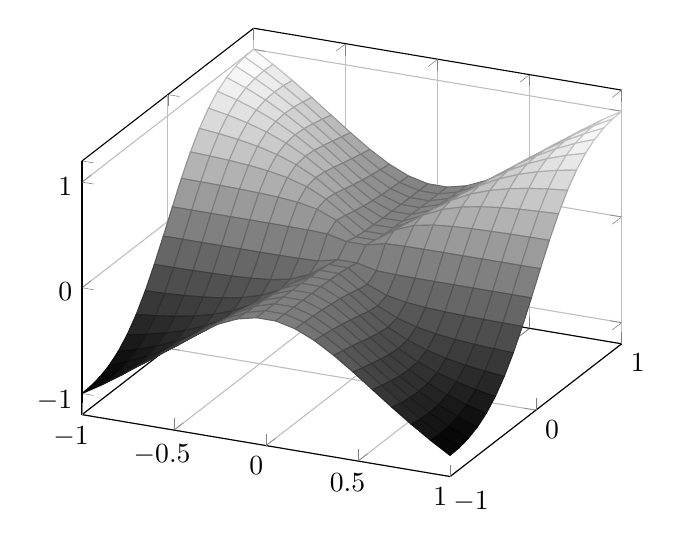
\begin{tikzpicture}
		\begin{axis}[
			domain    = -1:1,
			samples    = 20,
			y domain  = -1:1,
			samples y  = 20,
			colormap/blackwhite,
			grid,
			]
			\addplot3[surf] { 2 * x^2 * y / (x^2 + y^2 ) };
		\end{axis}
	\end{tikzpicture}
	}\\
	\subfloat[Aufgabe 4]{
	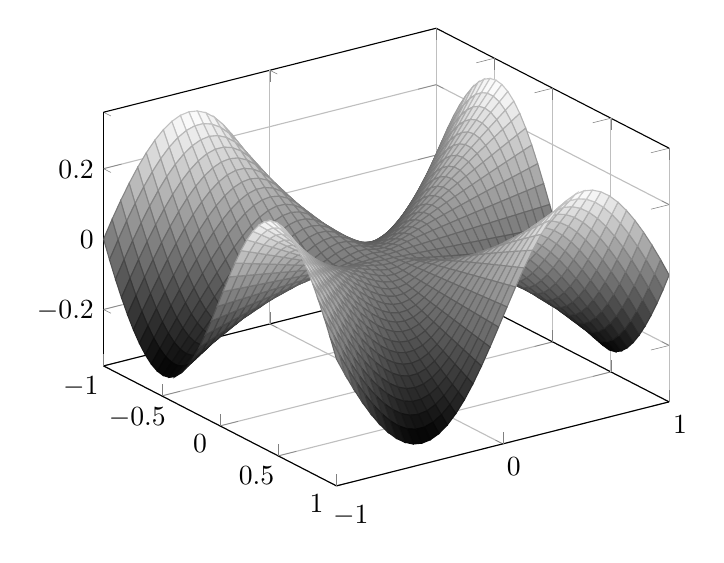
\begin{tikzpicture}
		\begin{axis}[
			domain    = -1:1,
			samples    = 40,
			y domain  = -1:1,
			samples y  = 40,
			colormap/blackwhite,
			grid,
			rotate around z = -30,
			]
			\addplot3[surf] { x * y * (x^2 - y^2) / (x^2 + y^2 ) };
		\end{axis}
	\end{tikzpicture}
	}
\end{figure}

\end{document}

